\documentclass[11pt]{article}

\usepackage[a4paper,margin=2.1cm]{geometry}
\usepackage{graphicx}
\usepackage{booktabs}
\usepackage{amsmath}
\usepackage{microtype}
\usepackage{caption}
\usepackage[hidelinks]{hyperref}
\usepackage{xcolor}
\usepackage{titlesec}

\captionsetup{font=small,labelfont=bf}
\titlespacing*{\section}{0pt}{0.8ex}{0.35ex}
\titlespacing*{\subsection}{0pt}{0.45ex}{0.15ex}
\titleformat{\subsection}{\normalfont\normalsize\bfseries}{}{0pt}{}
\titleformat{\section}{\normalfont\large\bfseries}{\thesection}{0.6em}{}
\setlength{\parskip}{0.15ex}
\makeatletter\newcommand\tablerows[1]{\@@input #1 }\makeatother

\title{\vspace{-1.2cm}\textbf{GridLink, Error Correction over a Screen-to-Camera Optical Channel}}
\author{COMP0228 Coursework 1, Group Report\\
\small Muhammad Maaz, Kanav Mehta}
\date{\vspace{-1.5ex}\small November 2026}

\begin{document}
\maketitle

\section{The communication channel}
We built GridLink, a one-way optical link from a laptop screen to a camera, one of the brief's
suggested channels and a small-scale relative of visible-light communication and screen-camera
links such as PixNet and COBRA \cite{haas,pixnet,cobra}. The transmitter fills a screen patch
with white for 1 and black for 0, one symbol at a time. The receiver records the patch through
an OpenCV camera, in most sessions not directly but via an iPad screen used as a mirror, whose
glossy surface reflects room light back as glare. Other sessions used a direct view or an
external monitor, and the path is recorded with each run. The channel is cheap, needs no extra
hardware, and mixes several physical noise sources (sampling jitter, auto-exposure, ambient
light and glare, drift), so the \emph{kind} of noise, not just its amount, can be studied.

\subsection*{Binary to signal and back}
The receiver measures mean brightness inside a calibrated region and thresholds it at the
midpoint of reference black and white levels; a run is rejected if contrast is too low. The
camera and screen clocks are independent and the camera delivers only 28 to 33 frames per
second in our captures, so the channel is a \emph{sampling} problem in the sense of this module.
At 8\,bps there are about four camera samples per symbol, at 2\,bps about fourteen. The
receiver timestamps every frame and takes the sample nearest each symbol centre (binary search
over sorted timestamps); missing observations stop decoding rather than silently becoming bits.

\subsection*{Framing}
Each message is a self-describing frame (\texttt{protocol.py}): a 48-bit sync word (alternating
preamble plus magic bytes), a 6-byte header (version, code, repetition factor, sequence, length)
with its own CRC-16, and the coded payload with a payload CRC-16. The header is always sent with
repetition-3, so 240 bits of fixed overhead. The receiver finds the sync word allowing up to 9
flipped bits, decodes the header, then the payload, and checks the CRC. The CRC detects but
cannot repair residual damage, which is what would enable retransmission (ARQ) in a two-way
link \cite{kurose}; we therefore always report failure counts alongside bit-error rates.

\section{Error-correcting codes}
All codes are pluggable encoders and decoders (\texttt{coding/}) with 40 unit tests, including
an exhaustive check that Hamming corrects every single error in every codeword and miscorrects
every double error. Each code trades rate for reliability; Shannon's theorem says reliable
communication is possible at any rate below capacity \cite{shannon}, and these simple codes sit
far from that bound, which is why the trade-off is so visible here.

\textbf{Repetition, N = 3, 5, 7.} Each bit is sent N times in a row and majority-voted, rate 1/N,
correcting up to $\lfloor N/2\rfloor$ flips per bit if they are not concentrated in one group.
\textbf{(7,4) Hamming} \cite{hamming}. Four data bits and three parity bits (rate 4/7); the
3-bit syndrome names the flipped position, so one error per codeword is corrected and two errors
are always miscorrected into three. \textbf{2-D parity, our third code.} Following the Kurose
and Ross exercise \cite{kurose}, 16 bits form a $4\times4$ grid with even row and column parities
($5\times5$, rate 16/25). A single error is located by its failing row and column; any other
failing pattern is rejected rather than guessed, trading Hamming's eager correction for honest
detection.

\section{Experimental method and statistics}
Experiments are scripted (\texttt{plan}, \texttt{record}, \texttt{transmit-plan},
\texttt{analyse}). A plan fixes payloads, codes, repeats, bit rate and a random seed; the seed
regenerates an identical shuffled schedule on the transmitter, so the two laptops never exchange
files and method order is randomised against drift. Each run stores raw brightness, decoded
results and physical conditions. We report channel BER (wrong observed frame bits), decoded BER
(complete decodable trials only), useful throughput (delivered payload bits per nominal frame
airtime) and frame success (decoded trials over planned trials). Methods are compared only within
a slice that shares bit rate, payload and environment. Every number, table row and figure in
this report is regenerated from the per-trial CSVs by one script (\texttt{report/make\_figures.py}).

With three trials per cell, the statistics have to be chosen with care. Frame success gets
Wilson 95\% intervals \cite{wilson}, which stay meaningful at 0/3 and 3/3 where the usual normal
interval collapses to a point. BER intervals use a bootstrap that resamples \emph{whole trials}
\cite{efron}, because errors within a frame are correlated (Section~5) and a per-bit binomial
interval would overstate our certainty. Method comparisons use Fisher's exact test. Questions
about noise structure use thousands of bits instead, through a permutation test and likelihood
model comparison (BIC).

\section{Results of the basic codes}
\textbf{Low noise (4 bps, mirror, Table~\ref{tab:clean}).} Channel BER is near zero and every
code, including uncoded, reaches decoded BER 0. Throughput then follows code rate, except that
Hamming lost one of three frames, so on a clean channel redundancy only costs rate.

\begin{table}[t]
\centering\small
\caption{Low-noise slice (4 bps, mirror, 16-bit payload). Every decoded BER is 0. Brackets give
Wilson 95\% intervals on frame success.}
\label{tab:clean}
\begin{tabular}{@{}lccc@{}}
\toprule
Method & Rate & Throughput (bps) & Frames [95\% CI] \\
\midrule
\tablerows{generated/table-clean.tex}
\bottomrule
\end{tabular}
\end{table}

\begin{table}[t]
\centering\small
\caption{High-noise slice (8 bps, direct screen). Decoded-BER brackets are trial-bootstrap
95\% intervals, frame brackets Wilson 95\% intervals.}
\label{tab:fast}
\begin{tabular}{@{}lcccc@{}}
\toprule
Method & Ch.\ BER & Dec.\ BER [95\% CI] & Thr.\ (bps) & Frames [95\% CI] \\
\midrule
\tablerows{generated/table-fast.tex}
\bottomrule
\end{tabular}
\end{table}

\begin{figure}[t]
\centering
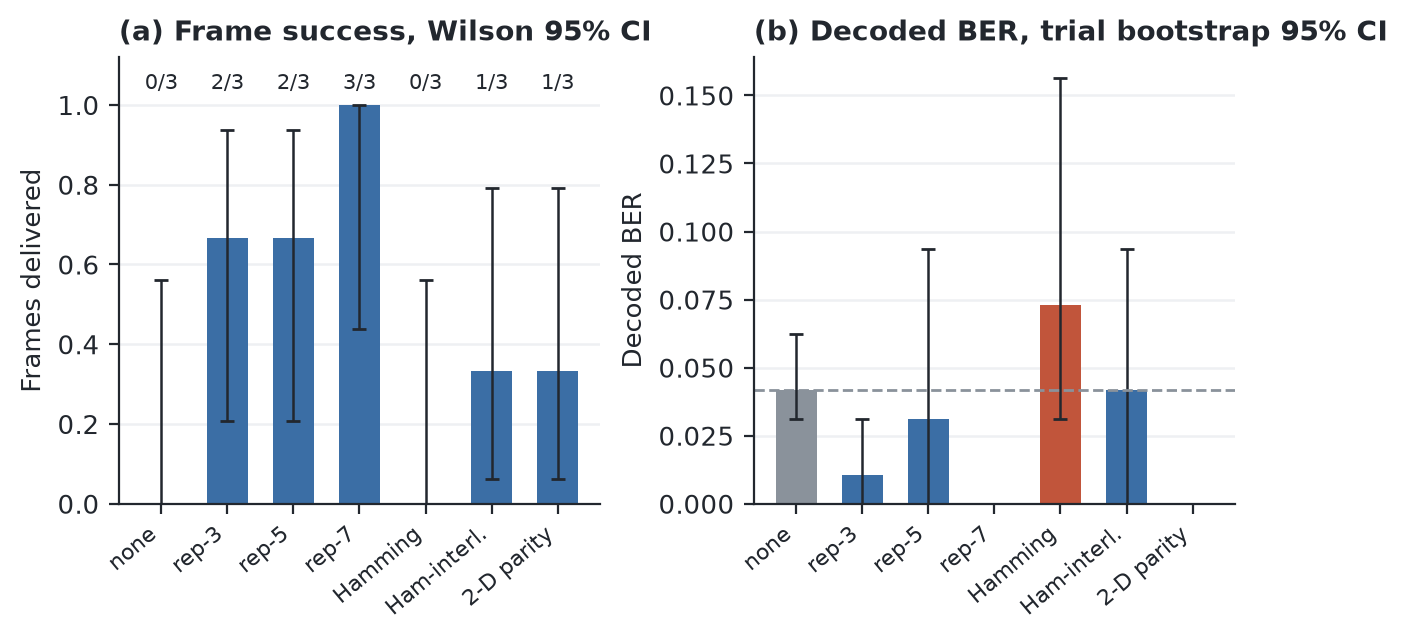
\includegraphics[width=\linewidth]{figures/highnoise-bars.png}
\caption{High-noise slice (8 bps, direct). (a) Frames delivered of 3, with Wilson intervals.
(b) Decoded BER with trial-bootstrap intervals; the dashed line is uncoded and red marks a code
that did worse than sending nothing.}
\label{fig:fastbars}
\end{figure}

\textbf{High noise (8 bps, direct, Table~\ref{tab:fast}, Fig.~\ref{fig:fastbars}).} Channel BER
rises to 3 to 5\%. Repetition-7 delivers 3/3 frames at zero decoded BER, but at one seventh of the
rate. Hamming's point estimate (0.073) is worse than uncoded (0.042): a 32-bit protected payload
is eight codewords, and at 5\% BER some carry two errors, which (7,4) turns into three. 2-D parity
never miscorrects (decoded BER 0) but rejects frames, delivering 1/3. These are the expected
trade-offs between correction power, residual error and delivery, but we state the uncertainty
plainly. The intervals overlap widely, and even the starkest contrast, repetition-7 3/3 against
Hamming 0/3, has Fisher $p=0.10$. Pooling the three seven-method sessions (9 trials per method),
frame success ranges from 4/9 uncoded to 8/9 for repetition-5, and no method differs
significantly from the best ($p\ge0.13$). Frame-level rankings are therefore suggestive only.
The decisive evidence comes from the bit-level analysis below, which uses thousands of bits.

\section{What kind of noise is this}
\textbf{Bursty or memoryless?} For each slice we compare the share of errors that sit in runs of
three or more with a null in which each trial's errors are scattered uniformly over its observed
bits (5000 permutations). Under glare, 87\% of errors are in such runs against 12\% under the null
($p<0.001$). At 8\,bps errors are mostly isolated, but even there 7.3\% are in runs against 0.6\%
($p<0.001$). At 3\,bps none are ($p=1$). A two-state Gilbert--Elliott model
\cite{gilbert,elliott}, a hidden Markov chain switching between a Good and a Bad state fitted by
Baum--Welch \cite{rabiner}, is strongly preferred over a memoryless channel by BIC for glare
(2261 against 3824) and modestly at 8\,bps (2174 against 2236). The glare fit has Bad spells
averaging 4.4 bits, occupying 12\% of the time, with nearly every Bad bit flipped. As a check on
a statistic it was not fitted to, the model reproduces the glare burst share (simulated 0.81,
95\% range 0.75 to 0.85, observed 0.87), whereas a memoryless channel at the same BER gives
0.05 (Fig.~\ref{fig:noise}b). At 3\,bps BIC also prefers the two-state model, but its ``Bad
spell'' lasts 923 bits, longer than a frame. That is not bursts but some trials simply being
noisier than others.

\begin{figure}[t]
\centering
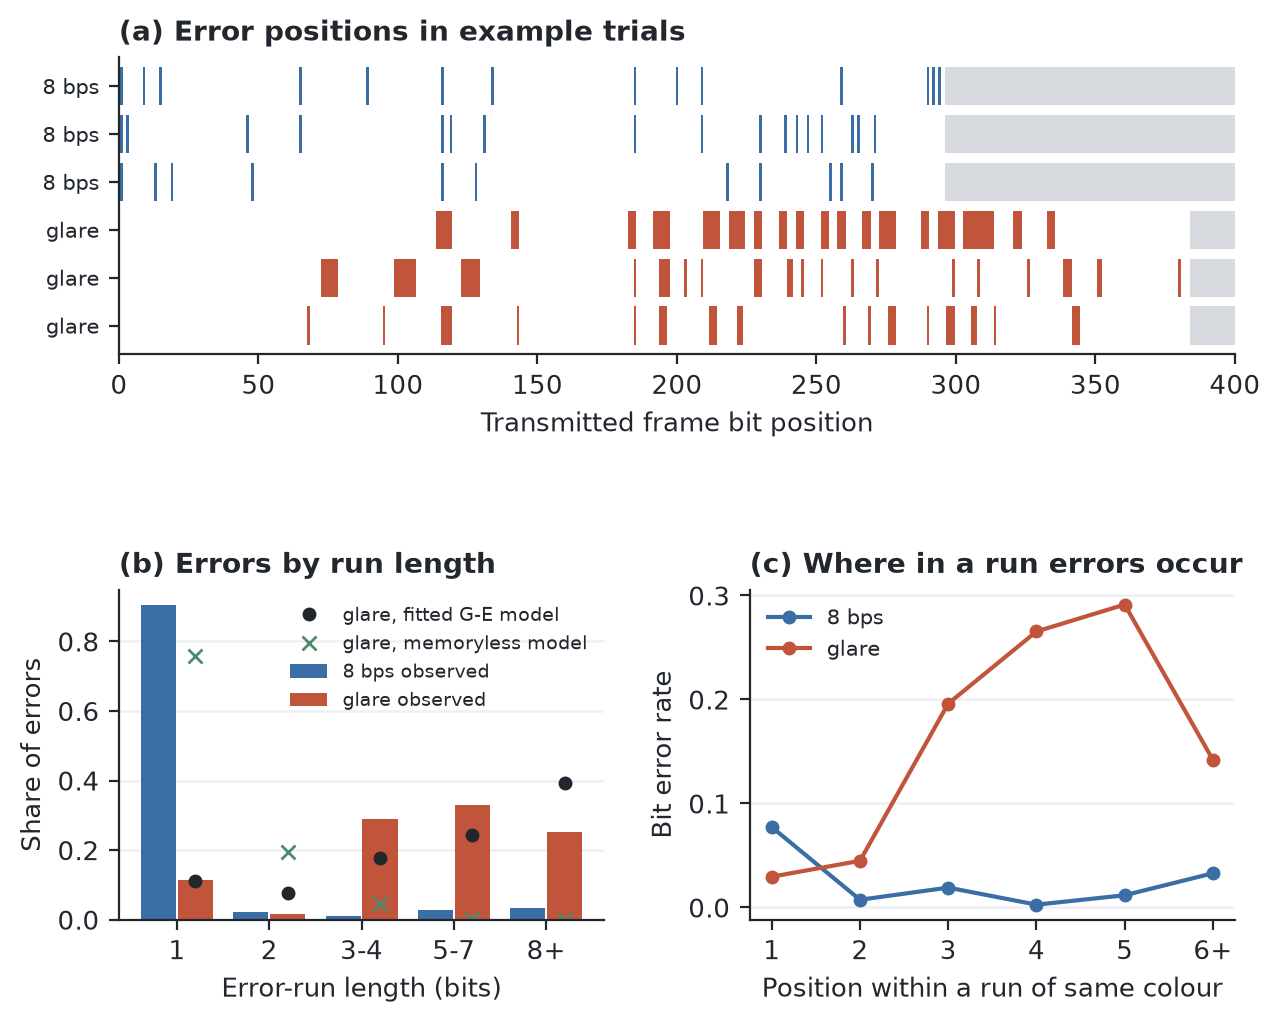
\includegraphics[width=\linewidth]{figures/noise-regimes.png}
\caption{(a) Error positions in example trials: 8\,bps errors are isolated, glare errors clump
(grey is unobserved). (b) Share of errors by error-run length, with the fitted Gilbert--Elliott
and memoryless models for glare. (c) Error rate against a symbol's position in a run of identical
colours: 8\,bps errors sit at the first symbol after a change, glare errors appear after a colour
has been held for three or more symbols.}
\label{fig:noise}
\end{figure}

\textbf{Two physical mechanisms.} Conditioning errors on the transmitted data separates the two
regimes (Fig.~\ref{fig:noise}c). At 8\,bps, 256 of 260 errors are black read as white, and a black
symbol fails 15.3\% of the time (130/850) right after a white one against 3.3\% (126/3794) after
another black (Fisher $p<10^{-10}$). White ``smears'' into the next symbol. With only about four
camera frames per symbol, an exposure straddling the edge or a small display-to-camera timing
offset reads the start of a black symbol as white, a form of intersymbol interference. Under
glare the pattern reverses. Errors are rare in the first two symbols of a run (62/1760, 3.5\%) and
common from the third onward (576/3232, 17.8\%, $p<10^{-10}$), on both colours. This fits the
camera's auto-exposure drifting while one colour is held, pushing the level across our fixed
threshold. A Gilbert--Elliott model whose error rate depends on run position fits glare better
still (BIC 2116): in a Bad spell, symbols early in a run flip with probability 0.23 and later
ones almost always. So the bursts are episodes in time that damage long same-colour runs.

\textbf{Are repetition and Hamming appropriate?} Both assume independent errors within a
codeword. The 8\,bps channel nearly meets that assumption, but at a BER where (7,4) Hamming is
overwhelmed. Glare breaks it badly. Of 624 repetition-3 groups, 77 had \emph{all three} copies
flipped, against 3.0 expected from a memoryless channel at the same BER, because adjacent copies
share one burst. Worse, repetition lengthens same-colour runs, which is exactly what triggers the
glare errors. Ten of the 15 glare failures were header CRC failures, so the payload code was never
reached, because the header uses the same adjacent repetition over mostly zero bytes. A further
confound follows from the 8\,bps mechanism. Channel BER depends on how often the data switches
colour, so repetition-7's low channel BER (0.016) partly reflects its fewer transitions, not
better luck.

\section{Extension: placing redundancy where the bursts are not}
\textbf{Hamming interleaving.} Guided by the burst finding, \texttt{hamming-interleaved} sends up
to eight (7,4) codewords column-first, so a burst of $b\le8$ consecutive bits hits each codeword at
most once. It costs no extra bits, the same idea as the cross-interleaved Reed--Solomon coding
that lets a CD survive scratches \cite{reed,immink}. Physically, interleaving matched Hamming on
the clean slice (3/3 against 2/3) and at 8\,bps delivered 1/3 against 0/3 with decoded BER 0.042
against 0.073. The intervals overlap, so we claim \emph{no} detectable physical difference. That
is what the noise analysis predicts, since 8\,bps errors are mostly isolated, and interleaving
only helps against bursts. In a synthetic test (Fig.~\ref{fig:ext}a, 400 trials per length,
identical burst positions for both Hamming variants) interleaving holds zero decoded BER up to its
depth of 8, while Hamming and repetition-3 fail from length 2 (0.072 and 0.042 at length 8).
Beyond about 13 bits it is worse than plain Hamming (0.184 against 0.144 at 16), because it then
spreads damage into more words.

\begin{figure}[t]
\centering
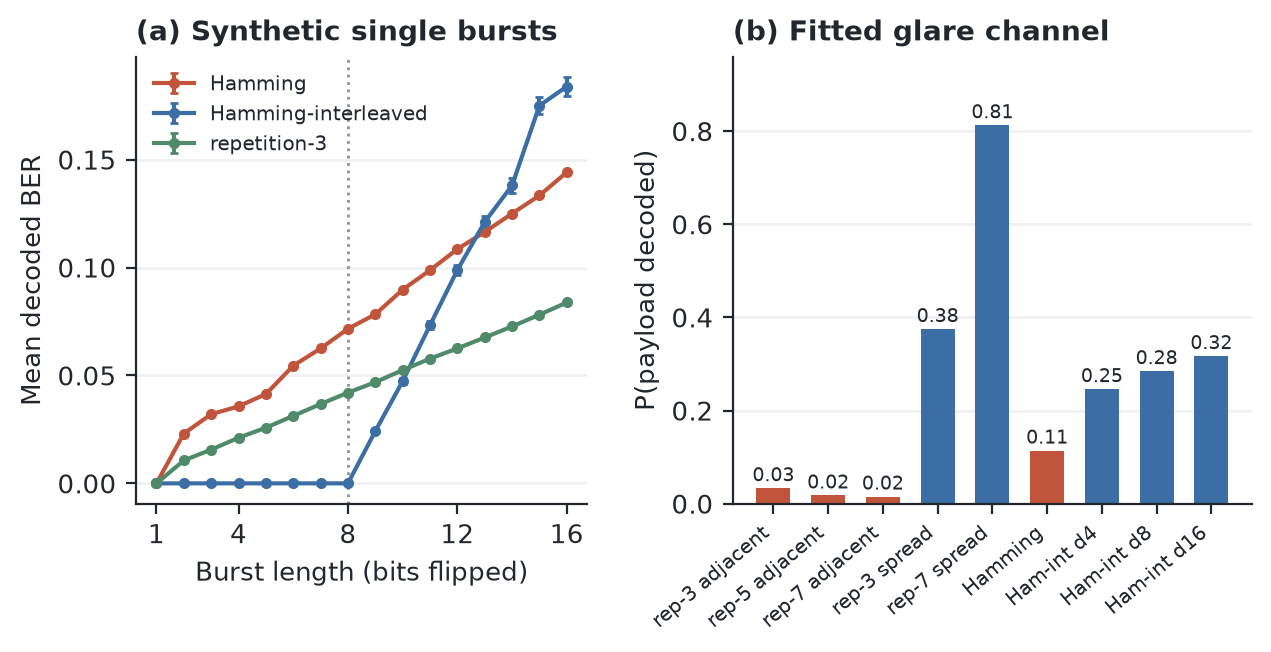
\includegraphics[width=\linewidth]{figures/extension.png}
\caption{(a) Synthetic single bursts, 64-bit payload, 400 trials per point, error bars one
standard error; dotted line marks interleaver depth 8. (b) Payload decoding probability on the
Gilbert--Elliott channel fitted to our glare data, 3000 simulated 4-byte frames per design. Red
is the built layout, blue a rearrangement at the same rate except where the copy count changes.}
\label{fig:ext}
\end{figure}

\textbf{Model-guided design on the fitted glare channel.} A single synthetic burst is not our
channel, so we used the fitted glare model to simulate whole frames through sync, header and
payload exactly as the receiver decodes them (Fig.~\ref{fig:ext}b, \texttt{design\_sim.py}). Three
results follow.
\begin{itemize}
\item \emph{Placement beats quantity.} With copies adjacent, adding redundancy makes things
worse (payload success 0.033, 0.018 and 0.015 for repetition-3, 5 and 7), because longer runs
mean longer bursts. Sending the whole message three times instead, at the same rate, gives 0.375,
and seven spread copies give 0.81.
\item \emph{Interleaver depth.} Payload success rises from 0.114 with no interleaving to 0.246,
0.285 and 0.317 at depths 4, 8 and 16. With Bad spells averaging 4.4 bits, returns diminish
past depth 8, which supports our choice.
\item \emph{The header is the bottleneck.} As built, only 0.8\% of headers survive the fitted glare
channel. Spreading the header copies the same way raises this to 22\% and whole-frame success
for spread repetition-3 from 0.2\% to 8.6\%.
\end{itemize}
The same rearrangements still help, more modestly, on the 8\,bps model (spread repetition-3
payload success 0.913 against 0.835). In absolute terms the stationary model is pessimistic: it
predicts almost no glare frames as built, while we observed 2/15 (Wilson 0.04 to 0.38), because
glare also switches on and off \emph{between} frames (session G22 had two near-clean frames and
one with 80 errors). We therefore use it to rank designs, not to forecast exact rates.

\textbf{Slowing down.} The simplest lever was rate. Glare runs at 2\,bps had 5 errors in 1152
bits (0.4\%) and delivered 2/3 frames, against 2/15 at 4\,bps. Because exposure drift grows with
time held, this improvement more likely reflects milder glare in that single session as well as
more samples per symbol. One session cannot separate the two, so we flag it as a confound rather
than a result.

\section{Conclusions, trade-offs and limitations}
On a clean channel coding only costs rate. As noise rises, the right choice depends on its
\emph{shape}, which our analysis measured rather than assumed. Isolated, data-dependent flips at
high rate favour heavy repetition or rejection (2-D parity) over (7,4) Hamming, which
miscorrects. Glare produces bursts tied to long same-colour runs, and there the decisive variable
is where redundancy sits, not how much there is. Interleaving, spreading copies and protecting
the header the same way give large modelled gains at no rate cost. The two mechanisms also point
beyond error correction, towards a run-length-limited, DC-balanced line code such as 8b/10b
\cite{widmer} or Manchester, which bounds how long a colour is held, and an adaptive threshold.
These are the standard fixes in wired links for the same drift problem.

\subsection*{Limitations and threats to validity}
(i) Three trials per cell give wide intervals, and no frame-level difference is significant. The
bit-level conclusions rest on 5{,}000 to 7{,}000 bits per slice, but those bits are clustered
within frames, which our trial bootstrap and permutation tests respect. (ii) Conditions differ
between sessions (lighting, device path, glare strength), so we compare only within slices. Even
within a slice, channel BER depends on the transmitted pattern, so codes face slightly different
channels. (iii) The design study is simulated on a stationary model that misses frame-to-frame
switching. Its rankings, not its absolute values, are the claim. (iv) Offline alignment can fail
in the worst captures, so some ``errors'' may be misalignment.

\textbf{Next physical test.} Ten or more trials per cell under fixed glare, comparing as-built
against spread repetition, deep interleaving and a spread header. Then a 2 against 4\,bps
comparison within one session to separate rate from glare strength.

\begin{thebibliography}{99}
\small\setlength{\itemsep}{0pt}
\bibitem{kurose} J.~F. Kurose, K.~W. Ross, \emph{Computer Networking: A Top-Down Approach},
8th ed., Pearson, 2021; 2-D parity exercise,
\url{https://gaia.cs.umass.edu/kurose_ross/interactive/2d_parity.php}.
\bibitem{shannon} C.~E. Shannon, ``A mathematical theory of communication,'' \emph{Bell Syst.
Tech. J.}, 27, 1948.
\bibitem{hamming} R.~W. Hamming, ``Error detecting and error correcting codes,'' \emph{Bell
Syst. Tech. J.}, 29(2), 1950.
\bibitem{gilbert} E.~N. Gilbert, ``Capacity of a burst-noise channel,'' \emph{Bell Syst. Tech.
J.}, 39(5), 1960.
\bibitem{elliott} E.~O. Elliott, ``Estimates of error rates for codes on burst-noise channels,''
\emph{Bell Syst. Tech. J.}, 42(5), 1963.
\bibitem{rabiner} L.~R. Rabiner, ``A tutorial on hidden Markov models and selected applications
in speech recognition,'' \emph{Proc. IEEE}, 77(2), 1989.
\bibitem{wilson} E.~B. Wilson, ``Probable inference, the law of succession, and statistical
inference,'' \emph{J. Amer. Statist. Assoc.}, 22(158), 1927.
\bibitem{efron} B. Efron, R.~J. Tibshirani, \emph{An Introduction to the Bootstrap}, Chapman \&
Hall, 1993.
\bibitem{reed} I.~S. Reed, G. Solomon, ``Polynomial codes over certain finite fields,''
\emph{J. SIAM}, 8(2), 1960.
\bibitem{immink} K.~A.~S. Immink, ``Reed--Solomon codes and the compact disc,'' in \emph{Reed-Solomon
Codes and Their Applications}, IEEE Press, 1994.
\bibitem{widmer} A.~X. Widmer, P.~A. Franaszek, ``A DC-balanced, partitioned-block, 8B/10B
transmission code,'' \emph{IBM J. Res. Dev.}, 27(5), 1983.
\bibitem{haas} H. Haas, L. Yin, Y. Wang, C. Chen, ``What is LiFi?'' \emph{J. Lightwave
Technol.}, 34(6), 2016.
\bibitem{pixnet} S.~D. Perli, N. Ahmed, D. Katabi, ``PixNet: interference-free wireless links
using LCD-camera pairs,'' \emph{Proc. ACM MobiCom}, 2010.
\bibitem{cobra} T. Hao, R. Zhou, G. Xing, ``COBRA: color barcode streaming for smartphone
systems,'' \emph{Proc. ACM MobiSys}, 2012.
\end{thebibliography}

\section*{Appendix, all recorded runs}
Table~\ref{tab:all} lists every recorded run behind the slices above: monitor (screen shown on an
external monitor), direct (camera viewing the screen), mirror (via the iPad) and glare (the dim,
high-glare mirror stress test). Methods are comparable only within a shared bps, payload and
environment, and BERs must be read with the frames-delivered column.

\begin{table}[h]
\centering\footnotesize
\setlength{\tabcolsep}{4.5pt}
\caption{Every recorded run: bps, payload bits (pay), environment (env), code, planned trials
(tr), channel BER, decoded BER, useful throughput (thr, bps), frames delivered (ok).}
\label{tab:all}
\begin{tabular}{@{}lllllrrrrr@{}}
\toprule
Run & bps & pay & env & code & tr & ChBER & DecBER & thr & ok \\
\midrule
\tablerows{generated/allruns-rows.tex}
\bottomrule
\end{tabular}
\end{table}

\end{document}
